%*****************************************
% Lab 04: Logic Operations
%*****************************************
\chapter{Logic Operations}\label{logic}

\section{Purpose}

This lab develops a logic unit that includes eight different logic functions using \LE library items. This device will eventually be used as part of the \acf{ALU} in Lab \ref{alu}. This device will have two inputs, labeled \textit{A} and \textit{B}, and will output the following logic values.

\begin{enumerate}
	\item $ AB $
	\item $ (AB)' $
	\item $ A+B $
	\item $ (A+B)' $
	\item $ A Xor B $
	\item $ AB' $
	\item $ A+B' $
	\item $ A' $
\end{enumerate}

\section{Procedure}

This circuit is very similar to the arithmetic circuit developed in Lab \ref{arith}. However, the logic circuit is much simpler than the arithmetic circuit since there is not carry in/out bit and no comparator output.

To complete the lab, create a subcircuit named \lstinline[columns=fixed]|logic|. Place appropriate devices from the \textit{Gates} library in the \lstinline[columns=fixed]|logic| subcircuit. Connect each of the devices to inputs \textit{A} and \textit{B} and then wire the outputs from each device to \textit{LoOut} through a multiplexer. The exact design of the \lstinline[columns=fixed]|logic| subcircuit is left to the student.  

Drop the \lstinline[columns=fixed]|logic| subcircuit on the  \lstinline[columns=fixed]|main| circuit and wire the various inputs and outputs, as shown in Figure \ref{fig:logic-01}. 

\begin{figure}[H]
	\centering
	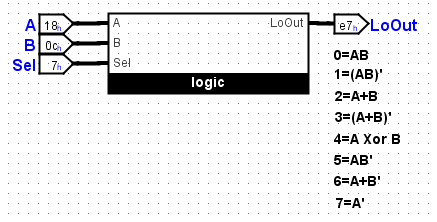
\includegraphics[width=\maxwidth{.95\linewidth}]{gfx/logic-01}
	\caption{The Main Logic Circuit}
	\label{fig:logic-01}
\end{figure}

The circuit can be tested by using the \textit{poke} tool and entering various inputs and then checking to see that the output is correct. A test vector files is also provided with the lab and that can be used to ensure the subcircuit is correct.

\section{Deliverable}

To receive a grade for this lab, complete the circuit. Be sure the standard identifying information is at the top left of the \lstinline[columns=fixed]|main| circuit, similar to: 

\bigskip
% The minipage environment keeps the three lines together - no page break.
\begin{minipage}{\linewidth}
	\begin{verbatim}
	George Self
	Lab 04: Logic Operations
	September 17, 2019
	\end{verbatim}
\end{minipage}
\bigskip

Save the file with this name: \emph{\texttt{Lab04\_Logic}} and submit that file for grading.

